\newchapter{c:phasePropagation}{Phase Propagation}

This is the introductory text.

\newsection{s:origJitter}{Characteristics of Uncorrected Phase Jitter}

\newsection{s:r56}{First Order Energy Dependencies}

\begin{figure}
  \centering
  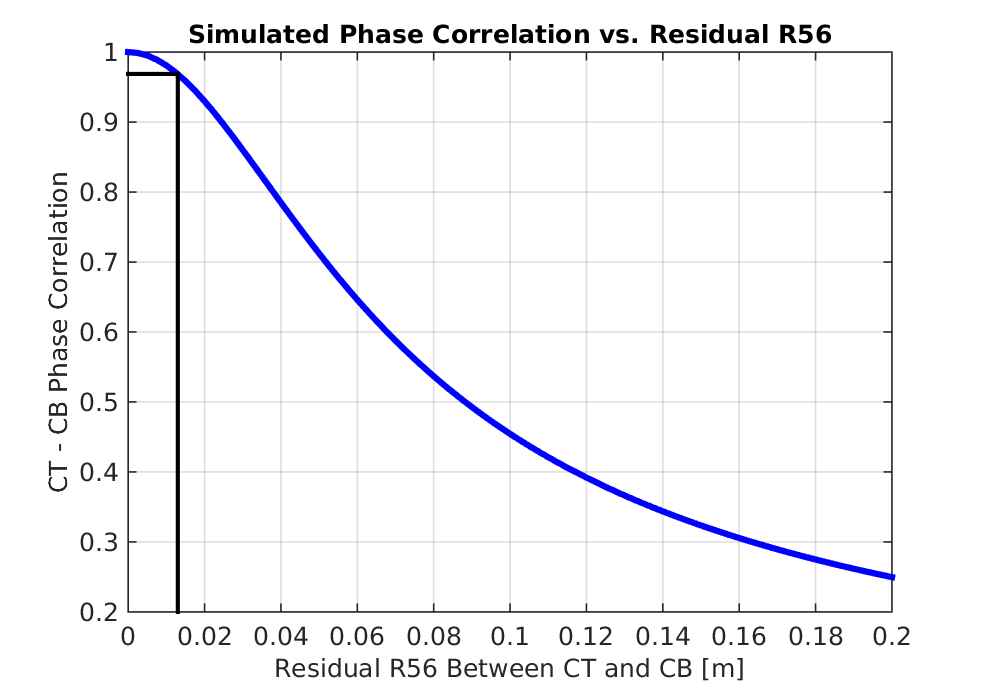
\includegraphics[width=0.45\textwidth]{Figures/R56_corrSim}
  \caption{Phase correlation vs. residual R56 between monitors.}
  \label{f:R56_corrSim}
\end{figure}

\newsection{s:t566}{Higher Order Energy Dependencies}

\begin{figure}
  \centering
  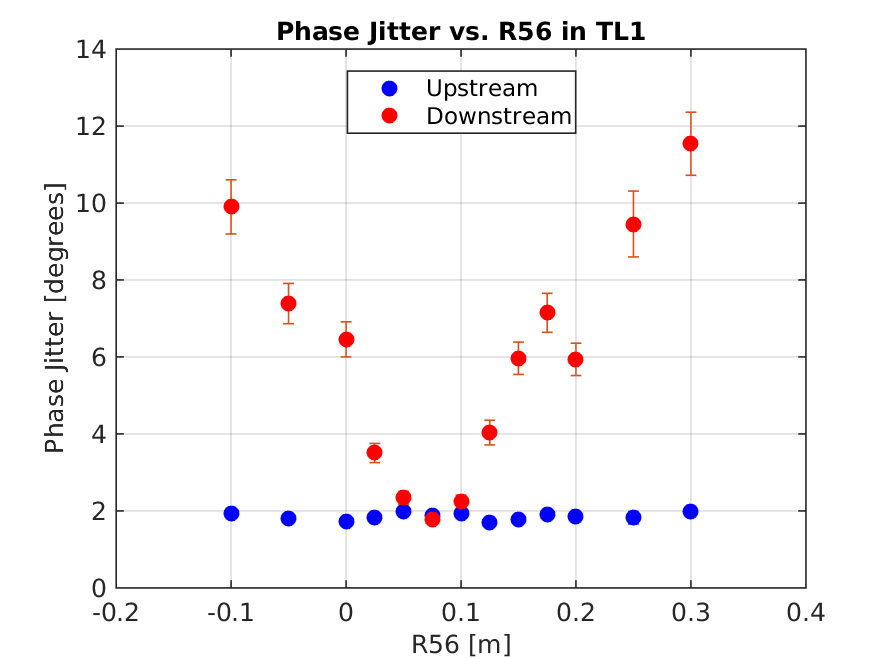
\includegraphics[width=0.45\textwidth]{Figures/R56ScanGunWiggle_PhaseJitter}
  \caption{Phase jitter for different R56 whilst wiggling gun current.}
  \label{f:R56ScanGunWiggle_PhaseJitter}
\end{figure}

\begin{figure}
  \centering
  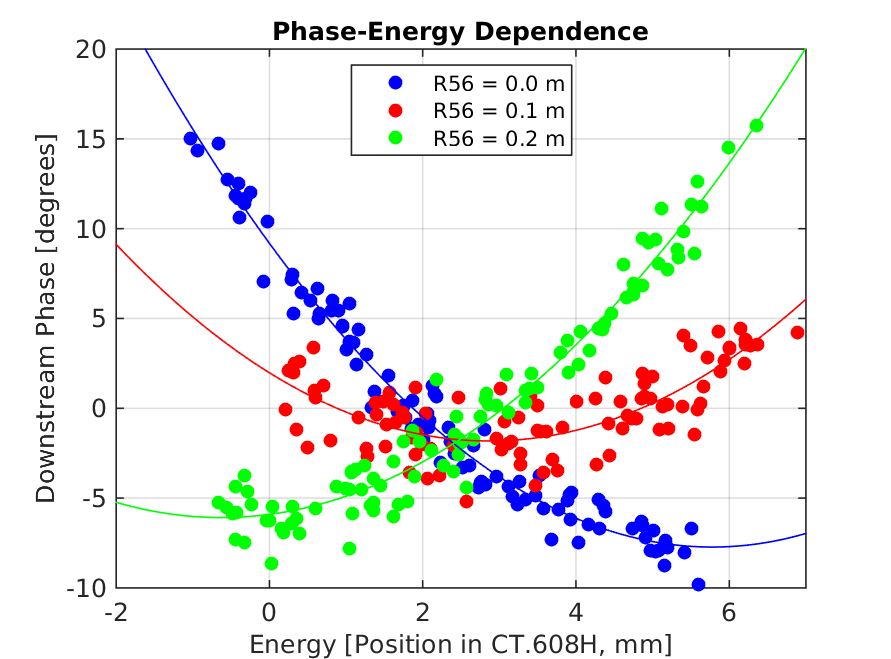
\includegraphics[width=0.45\textwidth]{Figures/R56ScanGunWiggle_Vs608}
  \caption{Phase vs. energy for different R56 in TL1.}
  \label{f:R56ScanGunWiggle_Vs608}
\end{figure}


\newsection{s:otherJitterSources}{Other Sources of Phase Jitter}

\newsection{s:longTermStability}{Long Term Propagation Stability}







